\section{Experiment}

\begin{SCfigure}
  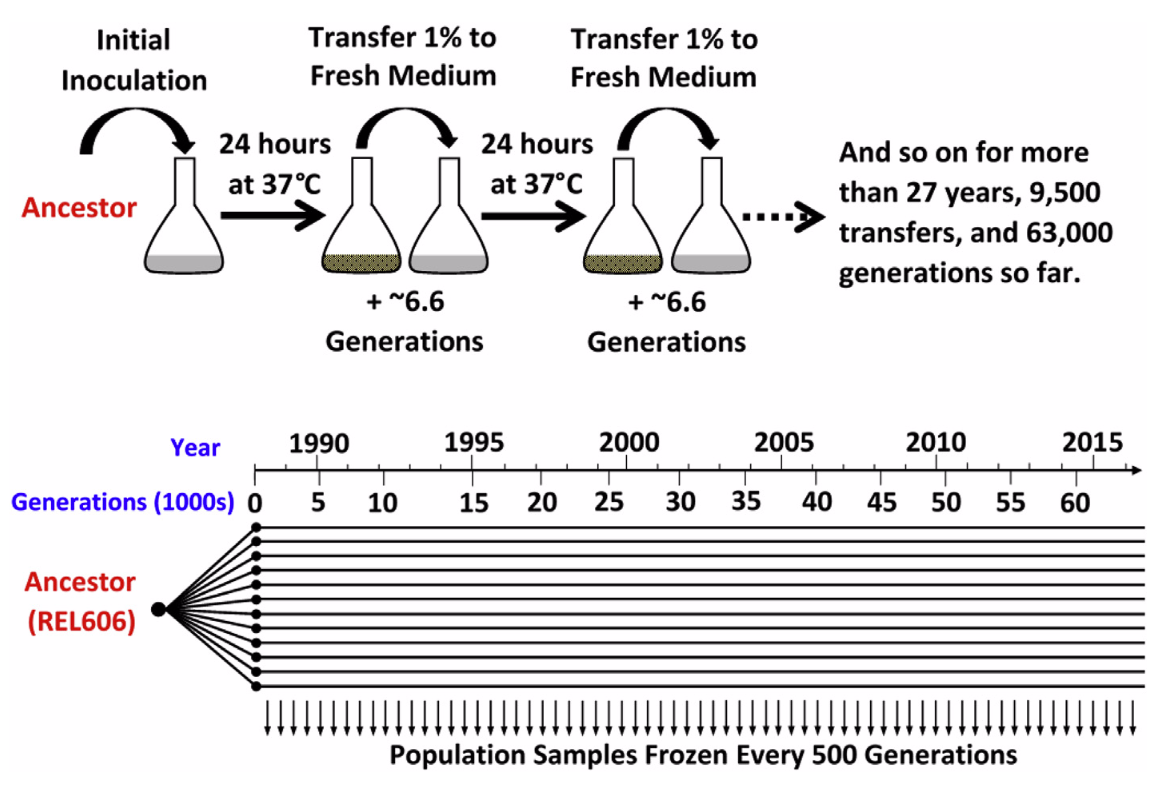
\includegraphics[width=0.7\textwidth]{img/ltee_schematic}
  %\captionsetup{singlelinecheck=off,justification=raggedright}
  \hspace{2ex}
  \caption[Overview of the Lenski \textit{E. coli} Long-Term Evolution Experiment]{In the LTEE, twelve \textit{E coli.} strains are propagated through daily serial transfers. Every 24 hours, during which time approximately 6.6 generations elapse, 1\% of the population is extracted and placed in fresh growth medium \cite[Figure 1]{Blount2016AContingency}.}
  \label{fig:ltee_schematic}
\end{SCfigure}

As depicted in Figure \ref{fig:ltee_schematic}, at its core the Lenski LTEE follows the parallel evolution of a dozen \textit{E. coli} lineages.
These lineages are maintained in separate liquid growth mediums. 
Daily transfers install a small fraction of the existing population in a fresh medium \cite{Blount2016AContingency}.
Every 500 generations, samples from the remaining population after transfer of \textit{E. coli} to fresh media are frozen away at \SI{-80}{\celsius} in glycerol \cite{Lenski2017TheSite}.
These biological archives allow for later detailed analysis of the genetic and phenotypic changes each lineage experienced over the course of the experiment \cite{Blount2012GenomicPopulation} and for critical evolutionary periods to be replayed in replicate \cite{Turner2015ReplayingPopulation}.

The B strain of \textit{E. coli} employed in the LTEE was selected for traits that make accounting for genetic material straightforward. 
The \textit{E. coli} strain chosen propagates exclusively through strict clonal descent --- the strain does not harbor plasmids or functional bacteriophages or reproduce sexually \cite{Lenski1991Long-TermGenerations}.
Hence, novel genetic traits can be attributed with high confidence to \textit{de novo} mutation events that occurred within the course of the experiment.
The strain also exhibits the handy characteristics of short generation time (approximately six generations per day), ability to be suspended indefinitely in glycerol at \SI{-80}{\celsius} and subsequently reanimated, and well-developed biological and procedural characterization due to its common use in laboratory experiments \cite{Lenski2017TheSite,Lenski1991Long-TermGenerations}.
Additionally, the strain selected was specifically sensitive to bacteriophage T5 and resistant to bacteriophage T6.
This property, which differentiates the B strain of \textit{E. coli} from other \textit{E. coli} and other bacteria, allows the LTEE lineages to be readily checked for cross-contamination \cite{Lenski2017TheSite}.

In the Lenski LTEE, E coli. are cultured in the Davis minimal broth, also known as DM25. 
Thiamine hydrochloride and glucose are added to the broth at 
concentrations of \SI{2e-6}{\gram\per\liter} and \SI{2.5e-2}{\gram\per\liter}, respectively \cite{Lenski1991Long-TermGenerations}. 
The glucose concentration was set so that the supply of this nutrient would be quickly exhausted by the growth of \textit{E. coli}.
Thus, the populations cycle daily between satiety and resource exhaustion \cite{Blount2016AContingency}.
Citrate, which turned out to represent a potential alternate food source for \textit{E. coli}, is present in the DM25 broth at a significant concentration of \SI{1700}{\micro\Molar}.
This amounts to more than ten times the concentration of glucose.
At the outset of the experiment, citrate was included simply  to conform to the established recipe for the DM25 broth \cite{Blount2016AContingency}.
The \textit{E. coli} B strain chosen by Lenski to found the LTEE's dozen lineages is incapable of aerobically metabolizing citrate, although \textit{E. coli} can ferment the compound in an Oxygen-poor environment \cite{Blount2016AContingency}.
This inability of \textit{E. coli} to metabolize citrate aerobically stems from the regulation of the citrate transporter CItT, which is exclusively expressed in anaerobic environments \cite{Pos1998TheChloroplasts}.

The B strain of \textit{E. coli} selected by Lenski et al. also did not exhibit an ability to metabolize the sugar L-arabinose.
At the outset of the experiment, a large number of cells of the strain screened for the ability to synthesize L-arabinose.
A colony of such cells was isolated.
The ability to metabolize L-arabinose proves a useful indicator.
Colonies capable and incapable of L-arabionse metabolization can be readily distinguished on tetrazolium arabinose indicator plates, with the former taking on a white color in contrast to the red color taken on by the latter.
Strains of \textit{E. coli} capable and incapable of metabolizing L-arabinose are described as Ara$^+$ and Ara$^-$, respectively \cite{Lenski1991Long-TermGenerations}
The original B strain of \textit{E. coli} acquired by Lenski et al. and the Ara$^+$ variant isolated from the original strain were specifically deemed REL607 and REL606, respectively \cite{Lenski2017TheSite}.
Although the Ara$^+$ strain uniquely exhibits the ability to metabolize L-arabinose sugar, the two strains were demonstrated to exhibit relative fitness of 1.00 +- 0.01 (95\% confidence interval) under the LTEE experimental conditions \cite{Lenski1988ExperimentalT4}.

Of the dozen lineages in the LTEE, six were founded from the REL606 strain and six were founded from the REL607 strain.
Maintaining both Ara$^+$ and Ara$^-$ lineages provides a methodological avenue for the assessment of fitness.
The fitnesses of two populations, one Ara$^+$ and the other Ara$^-$, relative to one another are assessed by:
\begin{enumerate}
\item growing each population separately in a liquid culture for a day,
\item mixing equal parts volume of both populations together in a fresh liquid medium and incubating for another day,
\item plating out the dual-population mixture on tetrazolium arabinose indicator plates, then
\item counting out colonies from each population based on the alternate colorations.
\end{enumerate} 
In the LTEE, three different types of fitness assessments were performed by placing clones from each of the evolved lineages in competition against baseline clones of the opposite Ara marker type and against clones from an alternate lineage within the same generational cohort of the opposite Ara marker type
\cite{Lenski1991Long-TermGenerations}.
In the course of the experiment, the Ara$^+$ and Ara$^-$ markers also provided a useful mechanism to detect inadvertent contamination.
Daily transfers strictly alternate between Ara$^+$ and Ara$^-$ strains \cite{Lenski2017TheSite}.
Periodic checks are made for cross-contamination between LTEE lineages using tetrazolium arabinose indicator plates \cite{Lenski1991Long-TermGenerations}.
At each daily transfer, backup copies of the lineage from the previous day are kept in the refrigerator to allow ready recovery in the event of a mishap \cite{Lenski2017TheSite}.


